\documentclass[]{auvsi_doc}
\setkeys{auvsi_doc.cls}{
	AUVSITitle={Airframe Component Placement},
	AUVSILogoPath={./../logo.pdf}
}

% include extra packages, if needed
\usepackage{tabularx}
\usepackage{booktabs}
\usepackage{longtable}

\begin{document}
	
	\begin{AUVSITitlePage}
		\begin{artifacttable}
			\entry{AF-014, 0.1, 03-01-19, SS Engineering Draft, Ryan Anderson, Tyler Critchfield}
			% additional \entry{} commands for extra rows in the revision table, if needed
		\end{artifacttable}
	\end{AUVSITitlePage}
	
	% document contents (see below for LaTex commands that make your life easier)
	\section{Introduction}
	To have a stable and aerodynamically efficient flight, it is vital that the airframe have a center of gravity (CG) at a specific location - specifically, one that is in front of the aerodynamic center (about 1/4 chord of the main wings). In our analysis of the airframe (see AF-011), we determined this location to be 6.2 cm in front of the leading edge of the wing. In this artifact, we present the locations of the major components of the system in order to achieve this desired CG of the entire aircraft. Figure \ref{fig:components} shows the placement of our main components in the airframe to achieve the desired CG. Table 1 lists the exact x-locations (measured from the nose of the aircraft) of each component. Only the x-location is listed because component placement primarily affects longitudinal stability (pitch). The y- and z-locations are not critical for our application. Note that only components with significant spacial requirements are included. This includes center of gravity, signal interference, and physical volume.
	
	%Begin table
	
	\begin{table}[h!]
		\begin{center}
			\caption{Layout of components for ideal CG placement, avoiding signal interference, and practicality.}
			\label{table:components}
			\begin{tabular}{p{1cm}p{2.5cm}p{4cm}p{7cm}}
				\toprule
				Item \# & X Location (cm) & Item Description & Reason for Location \\
				\midrule
				1 & 7.5 & GPS Antenna & Avoid interference with 5Ghz antenna \\
				2 & 17.5 & Ubiquiti Bullet & CG placement \\
				3 & 21.5 & Battery & CG placement \\
				4 & 33.5 & Camera & Near CG to reduce oscillations during image capture \\
				5 & 43.5 & Flight Controller and Inertial Sense & Inertial Sense should be near the CG  \\
				6 & 43.5 & Odroid & Central location is convenient for \newline connecting components \\
				7 & 52.5 & RC Antenna/Receiver & CG placement \\
				8 & 60.5 & UGV & CG placement, bay door design \\
				9 & 63 & 5GHz antenna & Avoid interference with GPS antenna \\
				10 & 68.5 & Parachute & Effective deployment with UGV \\
				\bottomrule
			\end{tabular}
		\end{center}
	\end{table}
	
	\begin{figure}[h!]
		\centering
		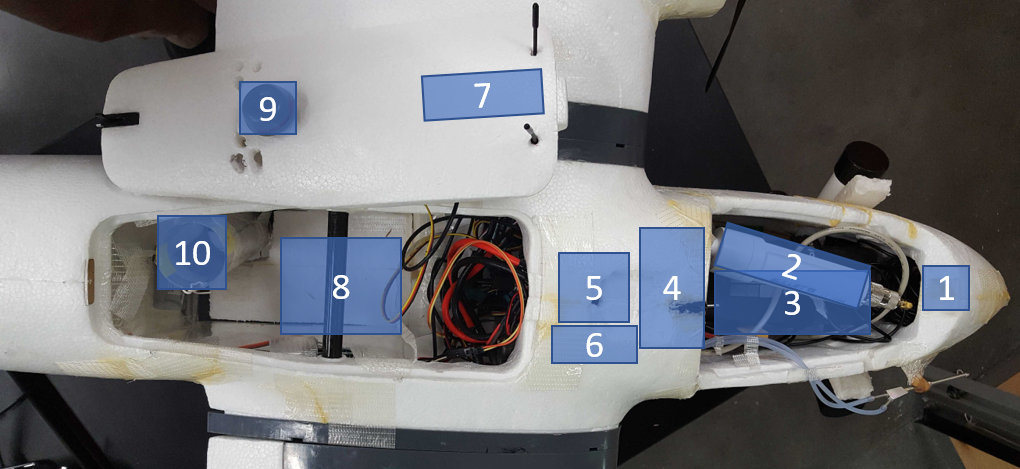
\includegraphics[width=.9\columnwidth]{figs/ComponentsPlacement.png}
		\caption{Diagram illustrating component placement. Numbers refer to those listed in Table 1.}
		\label{fig:components}
	\end{figure}
	
	
\end{document}
